%about objects not information; we can discuss in outside the box the issue of
%information needed forver but shuttled in and out.

\chapter{When It Won't Fit: Bulk Storage}
%\chapter{Extreme Scalability of Long-lived Data}
\label{chapter:large-long-lived}
\index{Bulk Storage}

% All of the tuning advice presented so far in this book can only get you so
% far.
There are limits to how well an object-oriented data model can scale.
At some point, you will be faced with the ineluctable limits of tuning objects.
Each object has its header, and this is an unavoidable cost. The only way to
avoid delegation costs, and thus amortize the cost of a header over more data
fields, is to go through the manual, iterative, process of inlining the fields
of one class into another. Some amount of this manual inlining makes sense, but
too much runs counter to principled engineering. Often, you are blocked because
you run into code that you do not own, or classes whose field layout is,
for one reason or another, set in stone.

In this way, a conventional storage strategy, one which maps entities to objects
and relations to collections, suffers from two problems that impact scaling up
the size and complexity of a design.

\paragraph{Amortizing away header costs.} Since entities are
  objects, and each object pays a header cost imposed by the \jre, you need to
  craft your design so that there is enough data in each object to amortize the
  cost of the headers, and to avoid high delegation costs.
 
\begin{wrapfigure}{r}{0.31\textwidth}
 \centering
 \vspace{-2mm}
 \begin{framedlisting}
 class X {
   A a;
 }
 class B extends A {
   int w, x;
 }
 class C extends A {
   int z;
 }
 \end{framedlisting}
 \caption{Delegation costs one object header, a cost that is easy to amortize.} 
 \label{fig:fragile-base-class}
\end{wrapfigure}
\paragraph{The Fragile Base Class problem.}
 %Any attempt to optimize, by
 %manually inlining the fields of one class into another, will likely suffer
 %from the fragile base class problem.
 \index{Fragile base class problem}
You may (wisely!) be unwilling to touch a class that is also used by other
 teams for fear of adversely impacting their correctness or
 memory footprint. For example, say class \class{X} delegates some of its
 behavior to an instance of class \class{A}, and that both \class{B} (your
 class) and \class{C} (the other team's class) are instances of \class{A}.
 %\autoref{fig:fragile-base-class} shows this example.
 Ignoring the other teams needs, you might prefer to collapse the fields of
 \class{B} into the \class{X} class, removing this need for delegation and that
 extra object header. To do so requires either modifying the implementation of
 \class{X}, or duplicating the implementation of \class{X} into a modified version of \class{B}. Neither alternative seems very appealing.
 This is a variant of what is known as the \emph{fragile base class problem}.

\begin{wrapfigure}[19]{l}{0.47\textwidth}
\centering
   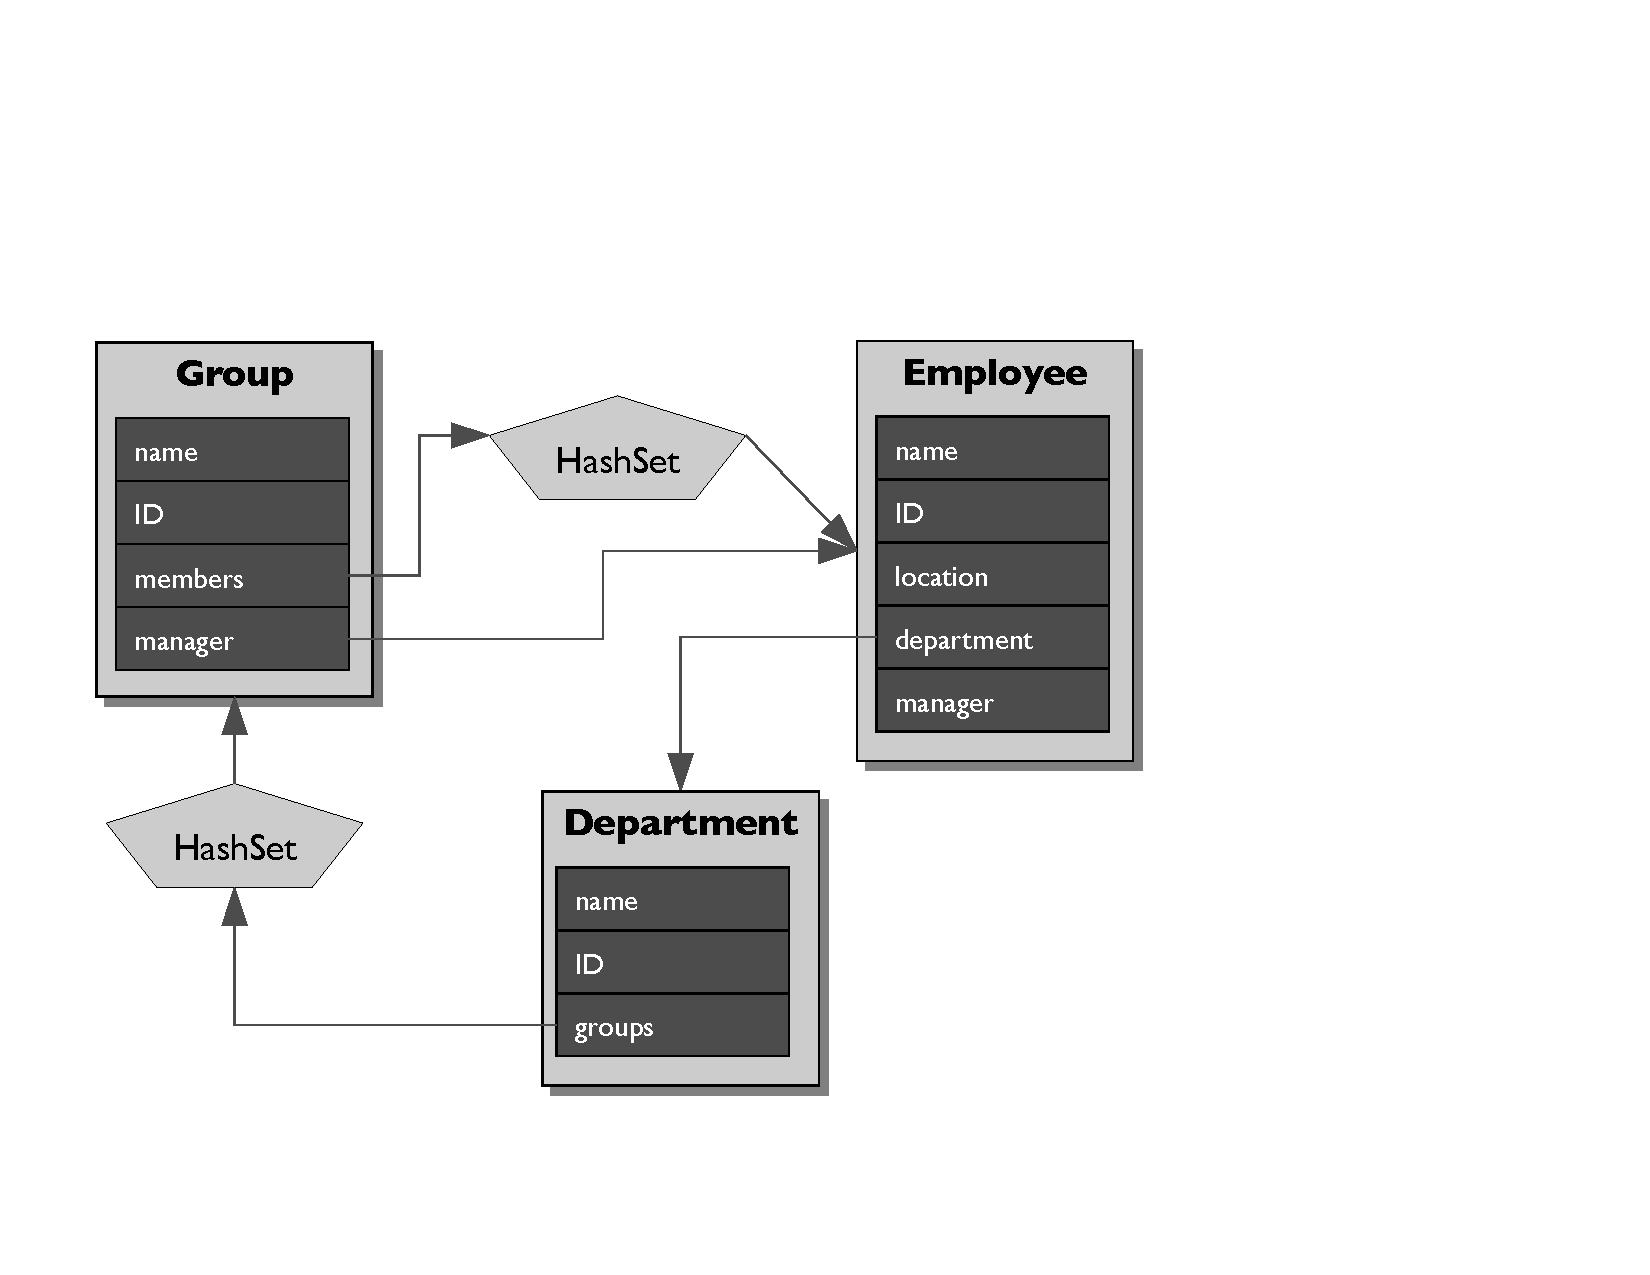
\includegraphics[width=0.46\textwidth]{part3/Figures/extreme/EC-example-for-columns1}
   \caption{A conventional storage strategy maps entities to objects, 
   attributes to fields, and relations to collections.}
   \label{fig:extreme-ec}
\end{wrapfigure}
If you break out of the Java mold, you may be able to overcome these issues. An
Entity-Collection diagram such as \autoref{fig:extreme-ec} maps pretty
inefficiently to a straightforward Java implementation. Each entity pays a
header cost, but has only a few data fields. Most of the collections,
representing relationships such as the number of employees under a manager, will
be small. 

\begin{wrapfigure}{r}{0.29\textwidth}
\centering
\vspace{-4mm}
\begin{framedlisting}
struct Node {
  enum Color color;
} nodes[20]
\end{framedlisting}
\caption{In C, \code{nodes} is an array of 20 integers, not
pointers to 20 separate heap allocations.}
\end{wrapfigure}
Storing data in bulk form means that the relations are stored in a small and
fixed number of collections, and the entities are stored in a small and fixed
number of objects --- across \emph{all} entities and relations between them.
They key is that the number of allocations is small and fixed, and therefore
object header overheads (and allocation costs) are easily amortized. The trick
to accomplishing a bulk storage approach is to store data in large arrays. This
can be accomplished in two ways: arrays of records and column-oriented storage.
\index{COBOL}
\index{Pascal}
\index{Arrays of records}
An array of records stores the fields of the entities back to back in the array,
without intervening pointers or headers. Arrays of records are not an option in
Java (they are in languages such as C, Pascal, COBOL, and C\#) and so this
chapter focuses on the latter approach: column-oriented storage.

% In a way that a graph of interconnected Java objects can never be, a bulk
% approach of storage is highly optimized for having a large number of entities.

\textbf{Warning!} Bulk storage violates some basic tenets of object-oriented
data modeling. Everything is a stored in an array, and thus there are no objects
to encapsulate the state of an individual entity. You will learn that
subclassing is more difficult to express, and
% Frthermore, these benefits to scalability come with some design costs, and
that a column-oriented approach may not suit the way your data is accessed and
updated.
% as discussed in \autoref{sec:when-bulk-storage-is-applicable}.
Nonetheless, with careful consideration of these issues, you can reap
substantial benefits.

%The main goals are to support a combination of flexibility and
%scalability that is not possible when following the precepts of object
%orientation.


%Sometimes, despite your best effors of tuning entities and collections, your
%application's objects still do not fit into the memory constraints of the
%target platform. 


%Managing a great number of long-lived objects therefore comes with its
%own set of challenges, even though objects these objects are free from the bugs
%that riddle those with correlated lifetime. To manage objects that, after a
%reasonable amount of tuning, still don't fit into the heap, you have three
%solutions at your disposal: throw hardware at the problem, implement a kind of
%demand paging, or code your data models in a non-object oriented way.

\section{Storing Your Data in Columns}
\label{sec:column-oriented}
\index{Column-oriented Storage}

In a column-oriented storage strategy, attributes are stored as arrays of data,
and an entity is implicitly represented by an index into these parallel
arrays. \autoref{fig:parallel-arrays} gives an example which takes the graph of
objects from \autoref{fig:extreme-ec} and represents the attributes of the
\class{Employee} entities in this fashion. Every group of entities, such as the
set of all employees, is stored in what amounts to a table of data. The range of
indices, 0 to 6 in this case, over the domain of attributes (\class{name},
\class{ID}, etc.), altogether represent what was previously a graph of
individual objects.

\callout{column-oriented}{Column-oriented Storage}{ A column-oriented strategy
stores everything, your data and the relations between them, as sets of parallel
arrays. Entities, rather than being individual allocations, are indicies into
these arrays.}

\index{Parallel arrays}
\begin{wrapfigure}{r}{0.3\textwidth}
\centering
\vspace{-5mm}
   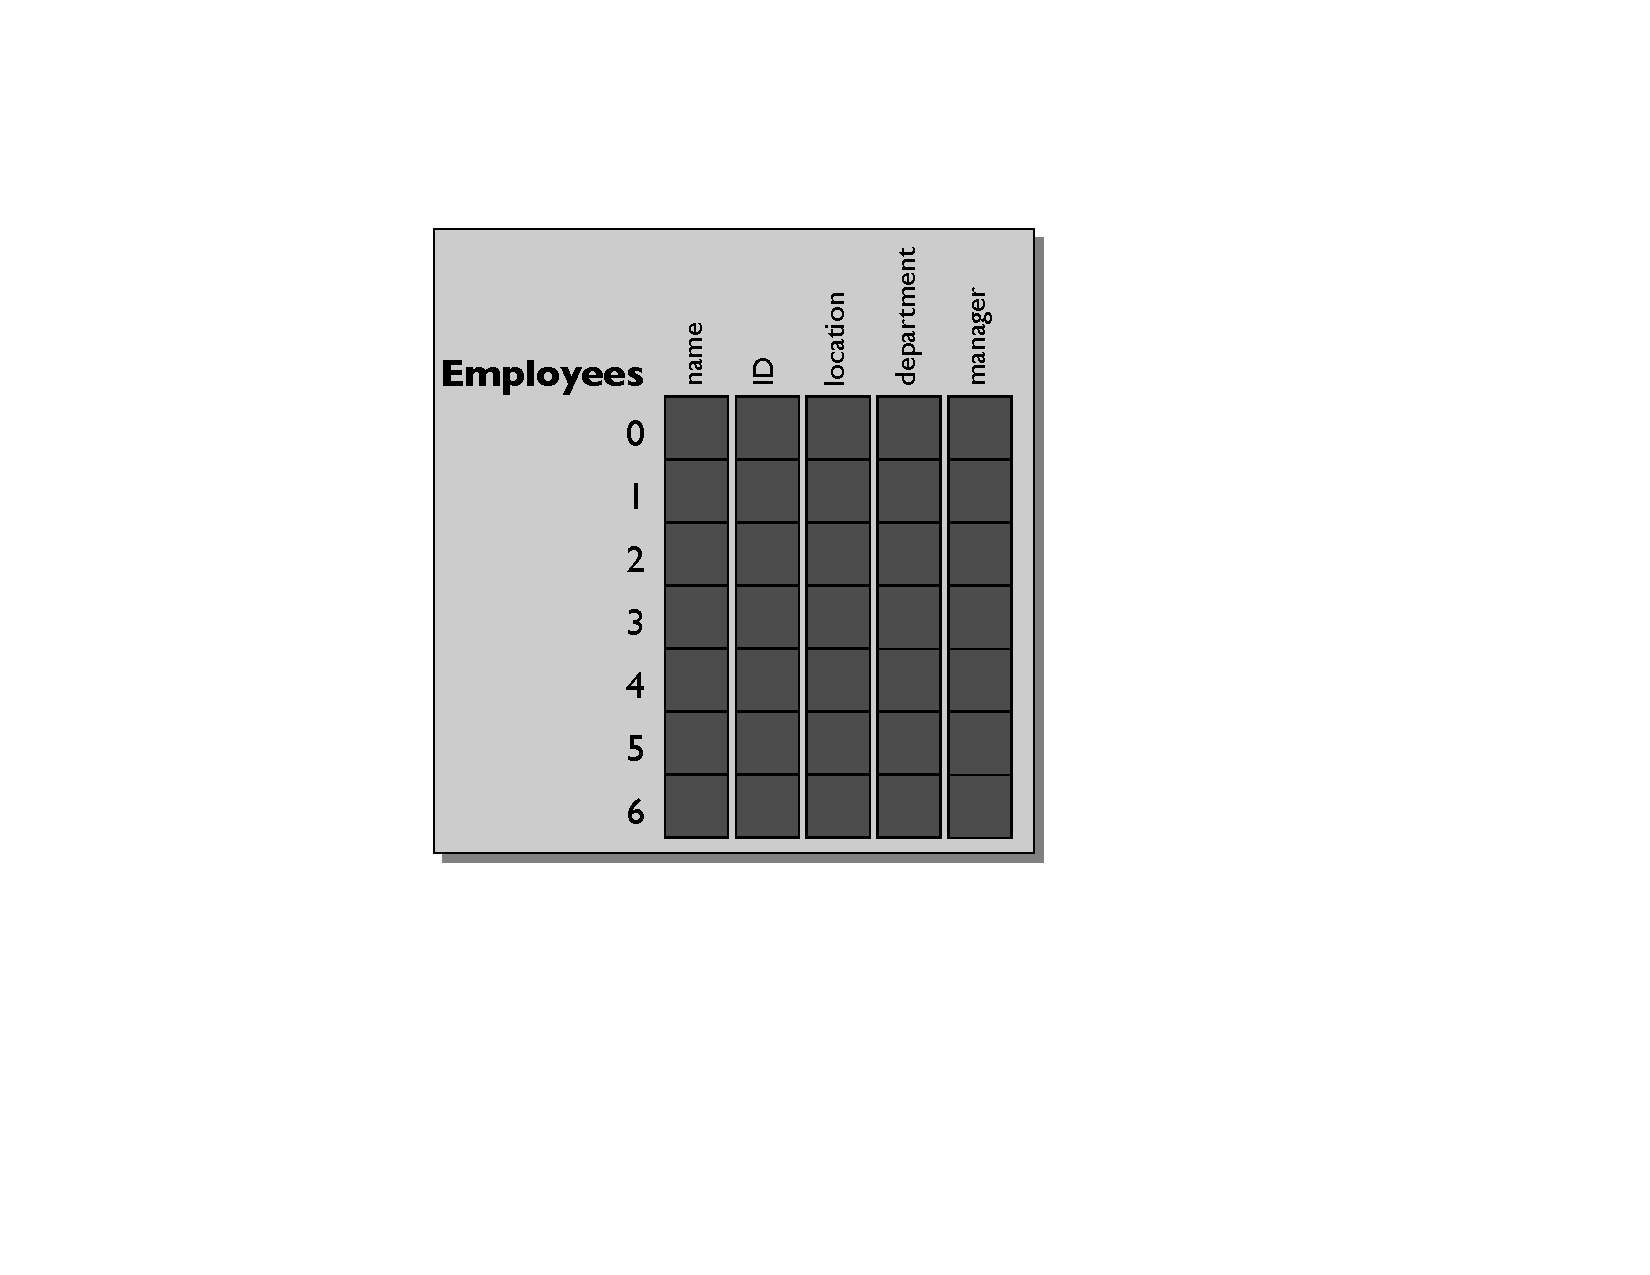
\includegraphics[width=0.28\textwidth]{part3/Figures/extreme/EC-example-for-columns2}
   \caption{Storing attributes in parallel arrays.}
   \label{fig:parallel-arrays}
\end{wrapfigure}
A column-oriented storage strategy consists of four tasks. First is storing the
primitive attributes of your entities, such as the \class{boolean} and
\class{int} data. Second is storing the relations between entities. Third is
storing variable-length attributes, such as string data. Finally is the task of
establishing the set of tables. There will be one per set of entities, one per relation between
entities, and one per source of variable length data. Let's step through these tasks now,
continuing the example from the previous chapter: storing a graph model.

\section{Bulk Storage of Scalar Attributes}
% (int, long, \ldots)
 
The example graph of the previous chapter finished with a bit of a condundrum.
You could store a flexible number of nodes and edges, but at high level of
memory bloat. Alternatively, by severely restricting the flexibility of the
implementation, could you achieve a pretty good level of scalability. Within the
normal confines of Java, these were the two choices. You should be able to
achieve a better balance by storing the graph in a bulk form.

\begin{wrapfigure}{l}{0.4\textwidth}
\vspace{-2mm}
\begin{framedlisting}
class Attribute<T> {
  T[] data;
  T get(int node) {
     return data[node];
  }
  int extent() {
    return data.length;
  }
}
\end{framedlisting}
\end{wrapfigure}
A graph model is a good candidate for storing in a column-oriented fashion.
Stored in this way, a graph without node attributes is simply one that has no
arrays to store node attributes. The is a direct correspondence between need for
and the existence of storage. This feature is hard to achieve in a purely
object-oriented approach, where having an interface for an entity at some point
demands that instances of that entity be created.

\autoref{fig:example-storing-relations-graph-with-node-numbers} repeats the
example graph from \autoref{fig:example-storing-relations-graph}, this time
including an identifier for each node. Each identifier is a natural number that
ranges, in this example, from 0--8 with no gaps. As far as node attributes are
concerned, the identifier of each node need not be stored anywhere. The figure
illustrates the identifiers for clarity, only. Once every node has been assigned
a dense identifier, then the attribute value of a given node attribute can be
stored and accessed in with that identifier.

\begin{wrapfigure}[16]{l}{0.525\textwidth}
\begin{framedlisting}
interface INodes {
  int numNodes();
}

class ColorNodes implements INodes {
  Attribute<Color> colors;
  
  int numNodes() {
    return colors.extent();
  }
  
  Color getColor(int node) {
    return colors.get(node);
  }
}
\end{framedlisting}
\end{wrapfigure}
% int getColor(int node) {
    % return colors.data[node];
  % }
In a column-oriented storage approach, rather than having interfaces and
implementations for individual nodes, you instead have them for a
\emph{set} of nodes. An instance of \class{INodes} 
defines the range of node indices for the nodes of that model, and includes
whatever combination of node attributes that you need for your given purpose.
If, for one use case, your nodes have colors, then you include that attribute in
your \class{INodes} model.

\paragraph{Freedom from Concensus Building}
If an object-oriented design is expected to be used by multiple groups, there is
usually a painful, iterative, process of reaching a concensus. Many groups, with
possibly competing trade-offs of time and space, and of what attributes are
necessary or optional, must reach a consensus as to how to lay out the data in a
class hierarchy.
Deciding which attributes belong in base classes versus
inherited classes, and of when to store attributes as fields or in a side
object, cannot be made in isolation, one group at a time. 

For the most part, these issues are much simpler when using column-oriented
storage. Adding new attributes to nodes or edges is a trivial operation. Adding
a new node attribute requires an extra array. You needn't reach a concensus
among developers as to whether this is a good idea.

\paragraph{Transient Need for Attributes}
If you only need node colors for the first phase of a multi-step algorithm, then
you can \code{null} out the colors attribute when you're done with it. This will
clear out all memory associated with that attribute. If the colors were spready
out into many individual node objects, rather than a single array, this would
require essentially reforming the entire graph. Assigning the color fields of
node objects to \code{null} would have no benefit, because in this case  the
color is a enumerated type.


%If the records of nodes are stored in
%an array called \code{nodes}, then
%to retrieve the color of the node
%with identifier 5 becomes \code{nodes[5].color}.

%Unfortunately, Java does not allow for arrays of structures. If the storage
%size of every field is known, and fixed, you can mimic this storage structure
%in Java, to a point. However, if your records have fields of varying types,
%this style of programming can boils down to doing the very same work you would
%do for marshalling data in and out of the Java heap. If the first and third
%attributes of your nodes are of \class{byte} size and the second is of
%\class{int} size, then accessing the third field of the node with identifier 5
% is
%tricky. It requires treating the entire record as a bit bucket, and shifting
%and masking appropriately.


%In this style
%of storage, you express collections of objects, rather than individual objects.
%The individuals are represented by indices. Instead of having a class for a
%node, you have a class for a group of nodes that participate, together, in a
%graph or several related graphs, as shown on the right.
%\autoref{fig:fortran-style} gives an example of a graph with 9 nodes.



\begin{wrapfigure}[9]{r}{0.46\textwidth}
\centering
\vspace{-3mm}
\begin{framedlisting}
class TransientNode {
  ColorNodes nodes;
  int node;
  
  Color getColor() {
    return nodes.getColor(node);
  }
}
\end{framedlisting}
\end{wrapfigure}
\paragraph{Transient Boxing}
Since individual nodes are now just numbers, you may quickly run into some
coding and maintenance problems. The Java compiler won't be of much use in
giving you static typing guarantees, because a node is an \class{int}
(serving as an index into arrays) just as much as integers that represent
other quantities. Imagine code where methods commonly have 5
\class{int} parameters, and trying to make sure you're passing the integer
values in the proper order.

\newcommand{\light}[1]{\footnotesize{\textcolor{Lighter}{#1}}}
\begin{figure}
\centering
\subfigure[Each node has an identifer.]{
\label{fig:example-storing-relations-graph-with-node-numbers}
	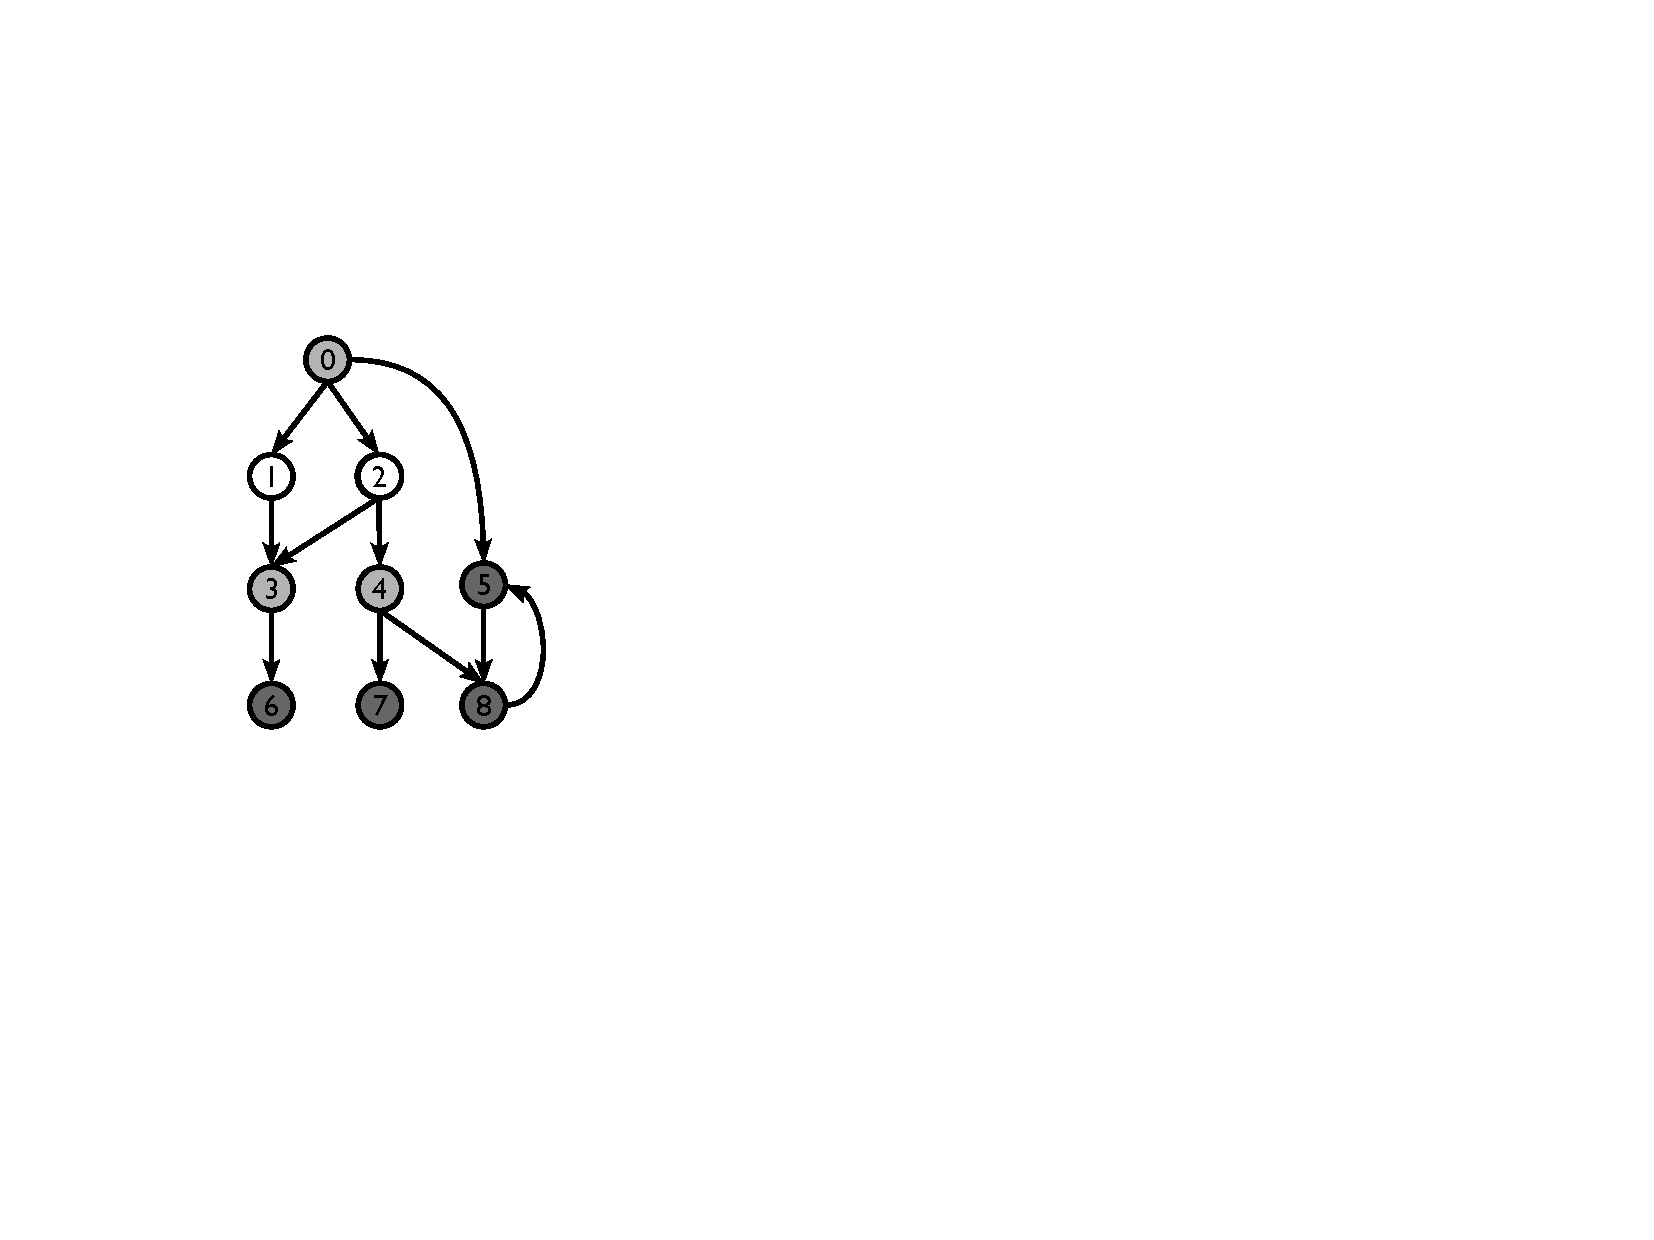
\includegraphics[width=0.3\textwidth]{part3/Figures/assessing/exampleGraph-withNodeNumbers}
	}
\quad
\subfigure[Node attribute.]{
\shortstack{
\begin{tabular}{ll}
\multicolumn{1}{r}{\light{id}} & \multicolumn{1}{l}{\textbf{Color}}
\\ \toprule
\light{0} & LightGray \\ \midrule
\light{1} & White \\ \midrule
\light{2} & White \\ \midrule
\light{3} & LightGray \\ \midrule
\light{4} & LightGray \\ \midrule
\light{5} & DarkGray \\ \midrule
\light{6} & DarkGray \\ \midrule
\light{7} & DarkGray \\ \midrule
\light{8} & DarkGray \\
\bottomrule
\end{tabular}
\\ \vspace{0mm}
}
}
\quad
\subfigure[The edges.]{
\shortstack{
\begin{tabular}{r@{~~$\rightarrow$~~}l}
\textbf{source} & \textbf{target}
\\ \toprule
0 & 1 \\
0 & 2 \\
0 & 5 \\ \midrule
1 & 3 \\ \midrule
2 & 3 \\
2 & 4 \\ \midrule
3 & 6 \\ \midrule
4 & 7 \\
4 & 8 \\ \midrule
5 & 8 \\ \midrule
8 & 5 \\
\bottomrule
\end{tabular}
\\ \vspace{0mm}
}
}
\caption{A graph of stored in 
 a column-oriented fashion.
%%Edge attributes, along with additional node attributes, would
%%be stored in additional columns.
%The \light{id} column is not a stored
%attribute, it is only shown for clarity.
%This edge table stores
%the source and target node indices. More compact storage is
%possible, as shown in \autoref{fig:fortran-style-edge-optimization}.
}
\label{fig:fortran-style}
\end{figure}

Using transient node facades can help here. Instead of passing around integers
to represent nodes, you can pass around temporary \class{Node} objects. As long
as manage the lifetime of these facades properly, being careful never to store
them in long-lived collections, then it is possible that you won't see a huge
performance hit by using them. With transient node facades, you are trading off
more time spent in garbage collection for convenience and the greater assurances
you get from strong typing. 

These transient node objects act as facades to the \class{INodes} model, and so
most store both a reference to the \class{INodes} model and the node's
identifier. Notice that these facades have two fields. If your nodes have only
one attribute, a purely object-oriented implementation would have only a single
field. Though it has one extra field, on top of the earlier node
implementations, for the \class{INodes} reference, as long as it is transient,
there is some chance that this won't result in an increase in garbage collection
overhead. This is something that requires experimentation in your setup. If
these result in big drags in performance for your use cases, remember that there
is no absolute need for these transient node facades.

You must also be careful to disallow, by convention, reference equality
checks against transient nodes. If you are not careful, you will need to persist
the transient facades, ruining any benefits of the column-oriented approach.
Similarly, if the lifetime of the facades is neither temporary, nor correlated
with a short-running method, you will certainly see negative impacts on garbage
collection overheads.

\section{Bulk Storage of Relationships}
\label{sec:bulk-storage-of-relationships}

\begin{wrapfigure}[17]{l}{0.36\textwidth}
\centering
\vspace{-3mm}
\begin{framedlisting}
class WeightedEdges {
  int[] source, target, weight;
  
  int source(int edge) {
    return source[edge];
  }
  
  int target(int edge) {
    return target[edge];
  }
  
  int weight(int edge) {
    return weight[edge];
  }
}
\end{framedlisting}
\end{wrapfigure}The edges of a graph can be represented as two parallel arrays, storing the
source and target node indices of each edge, as shown to the left.  
\autoref{fig:fortran-style}c illustrates a concrete example for a graph with 11
edges. For example, row number 4 represents the edge from node 1
to node 3. Any edge attributes, such as an edge weight, can easily be
represented as attributes parallel to the source and target arrays. 

This representation is a nice first step towards storing relations in a bulk
form, but it cannot efficiently support graph traversals. In order to traverse
the edges of a graph from a given node, you need to know the outgoing edges of a
given node.
% Even a \class{TransientEdge} class would not help, because
In this edge layout, the only way to get the outgoing edges of a node is to scan
the entire edge table, pulling out those rows whose \code{source} attribute
matches the given node identifier.

\paragraph{Indexing the Edges}
To allow for efficient traversals of the edges, you must index them, as a
database would. First, consider the outgoing edges from a node. If the
\class{source} and \class{target} arrays are sorted by the \textbf{source}
attribute, then all of the children of a node will be stored as contiguous rows.
This is a nice trick, and is what is shown in
\autoref{fig:fortran-style}c. 

Having sorted the edges, you can now leverage this property to allow for more
efficient traversal, as well as more efficient storage of the edge data. Notice
how the outgoing edges of node 2 start at row 5, and stop at row 6 (inclusive).
To visit the children of this node, without having to traverse the entire edge
model, you need to store these two row numbers somewhere. These two boundary
values, 5 and 6, are attributes of node 2. This means that a natural place to
store the edge index is as integer attributes in the node model; let's call
these \code{start} and \code{end}.

Also notice how the \code{source} attribute of \autoref{fig:fortran-style}c
contains lots of duplicate data; e.g. the two rows that represent the outgoing
edges of node 2 have the same \code{source} value (the value 2!). The
\code{start} and \code{end} node attributes, combined with the \code{target}
edge attribute is all you need to traverse the graph. 

Therefore, a more compact representation can eliminate the \code{source}
attribute entirely. \autoref{fig:fortran-style-edge-optimization} shows an
update to \autoref{fig:fortran-style}, where the node model now has, for the
outgoing edges, the two new attributes: \code{start} and \code{end}.


\begin{figure}
\centering
\subfigure[Node attributes. \code{start} and \code{end} are edge identifiers.]{
\shortstack{
\begin{tabular}{ll|ll|ll}
& & \multicolumn{2}{c|}{\textbf{Children}} &
\multicolumn{2}{c}{\textbf{Parents}} \\
\light{node id} & \multicolumn{1}{l|}{\textbf{Color}} &
\multicolumn{1}{l}{\textbf{start}} & \multicolumn{1}{l|}{\textbf{end}} & 
\multicolumn{1}{l}{\textbf{start}} &
\multicolumn{1}{l}{\textbf{end}} \\ \toprule
\light{0} & LightGray & 0  & 3 & -- & 0 \\
\light{1} & White     & 3  & 1 & 0  & 1 \\
\light{2} & White     & 4  & 2 & 1  & 1 \\
\light{3} & LightGray & 6  & 1 & 2  & 2 \\
\light{4} & LightGray & 7  & 2 & 4  & 1 \\
\light{5} & DarkGray  & 9  & 1 & 5  & 2 \\
\light{6} & DarkGray  & -- & 0 & 7  & 1 \\
\light{7} & DarkGray  & -- & 0 & 8  & 1 \\
\light{8} & DarkGray  & 10 & 1 & 9  & 2 \\
\bottomrule
\end{tabular}
\\ \vspace{0mm}
}
}
\qquad
\subfigure[Children edges.]{
\shortstack{
\begin{tabular}{ll}
\multicolumn{1}{r}{\light{edge id}} &
\multicolumn{1}{l}{\textbf{node id}} \\ \toprule
\light{0} & 1 \\
\light{1} & 2 \\
\light{2} & 5 \\ \midrule
\light{3} & 3 \\ \midrule
\light{4} & 3 \\
\light{5} & 4 \\ \midrule
\light{6} & 6 \\ \midrule
\light{7} & 7 \\
\light{8} & 8 \\ \midrule
\light{9} & 8 \\ \midrule
\light{10} & 5 \\
\bottomrule
\end{tabular}
\\ \vspace{0mm}
}
}
\quad
\subfigure[Parent edges.]{
\shortstack{
\begin{tabular}{ll}
\multicolumn{1}{r}{\light{edge id}} &
\multicolumn{1}{l}{\textbf{node id}}
\\ \toprule
\light{0} & 0 \\ \midrule  % 1 -> 0
\light{1} & 0 \\ \midrule  % 2 -> 0
\light{2} & 1 \\           % 3 -> 1
\light{3} & 2 \\ \midrule  % 3 -> 2
\light{4} & 2 \\ \midrule  % 4 -> 2
\light{5} & 0 \\ \midrule  % 5 -> 0
\light{6} & 8 \\           % 5 -> 8
\light{7} & 3 \\ \midrule  % 6 -> 3
\light{8} & 4 \\ \midrule  % 7 -> 4
\light{9} & 4 \\ \midrule  % 8 -> 4
\light{10} & 5 \\           % 8 -> 5
\bottomrule
\end{tabular}
\\ \vspace{0mm}
}
}
\caption{In order to support efficient traversal of the graph edges, you will
need to index them. These tables update the example of
\autoref{fig:fortran-style} to do so.  For example, node 2 has two children and
one parent. The children start at index 4 in
\autoref{fig:fortran-style-edge-optimization}b, which shows the two children to
be nodes 3 and 4.}
\label{fig:fortran-style-edge-optimization}
\end{figure}

\paragraph{Parent Edges}
The same thing can be done for the incoming edges, if we instead sort the edges
of \autoref{fig:fortran-style}c by the \textbf{to} attribute.
\autoref{fig:fortran-style-edge-optimization}a also shows the two new attributes
for the incoming edges.  For example, node 2 has two children and one parent.
The children start at index 4 in \autoref{fig:fortran-style-edge-optimization}b,
which shows the two children to be nodes 3 and 4.

%  used to have immutable in it
\section{Bulk Storage of Variable-length Data} %(e.g. Strings)}
\label{sec:bulk-sharing-pool}
\index{Bulk Sharing Pool}

The last remaining type of data is the strings and other data of variable
length. Storing a node or edge attribute in an array works well for any
attributes each of whose values is one of Java's primitive data types. If each
attribute value is an array, such as the case with string attributes, then a
single attribute array does not suffice. 

Even though the standard column-oriented storage strategy doesn't suffice, there
is still a big gain to be had to finding some way to store this data in a bulk
form.
% If your application has a few large primitive arrays, then the overhead of the
% arrays will be dwarfed by the actual data contained therein. A common
%In Java applications, a common problem is having many small primitive arrays.
%\index{Small Primitive Arrays}
If the length of an array is 10 characters, then it has a memory bloat factor of
61\%.
% 16/(10 + 16)
The problem grows worse if these primitive arrays are wrapped inside of objects
such as \class{String}. If wrapped inside of \class{String} objects, then your
the string has a bloat factor of 83\%.
% (16+32)/(10+16+32)
This is a pretty common problem, and so you should consider bulk storage of your
variable-length data, eve if you decide not to store your entities and relations
in bulk form.

There are several ways, within the constraints of Java, to avoid the object
headers of many small character arrays. One possibility is to use the built-in
string interning mechanism covered in
\autoref{sec:sharing-strings}\index{Interning}. By interning strings, your code
will pay for the string wrapper and the character array only once, rather than
once per occurrence of that string in the heap. Interning works well in reducing
overall heap consumption --- you're removing not only the many primitive array
object headers, but the entire content of duplicated arrays. As discussed in
that earlier chapter, you must pay careful attention, because interning is an
expensive process, and you only see reductions in memory footprint if there are
indeed duplicates to be found. 

\autoref{fig:bulk-sharing-pool}(a) and \autoref{fig:bulk-sharing-pool}(b)
illustrate a simple case of interning. Of three strings, there are two duplicate
``grape'' sequences. The residual high overhead is due to the remaining
primitive array object headers; all of the \class{String} objects are eliminated
by interning. Interning removes only the primitive array overheads of
\emph{duplicate} strings.

Of course, you can only use this built-in mechanism for \class{String} data. For
non-string data, or when there isn't much in the way of duplication, you can
still implement a solution that stores this data in a bulk form.

\begin{figure}
\centering
	\subfigure[Three normal	\class{Strings}.]{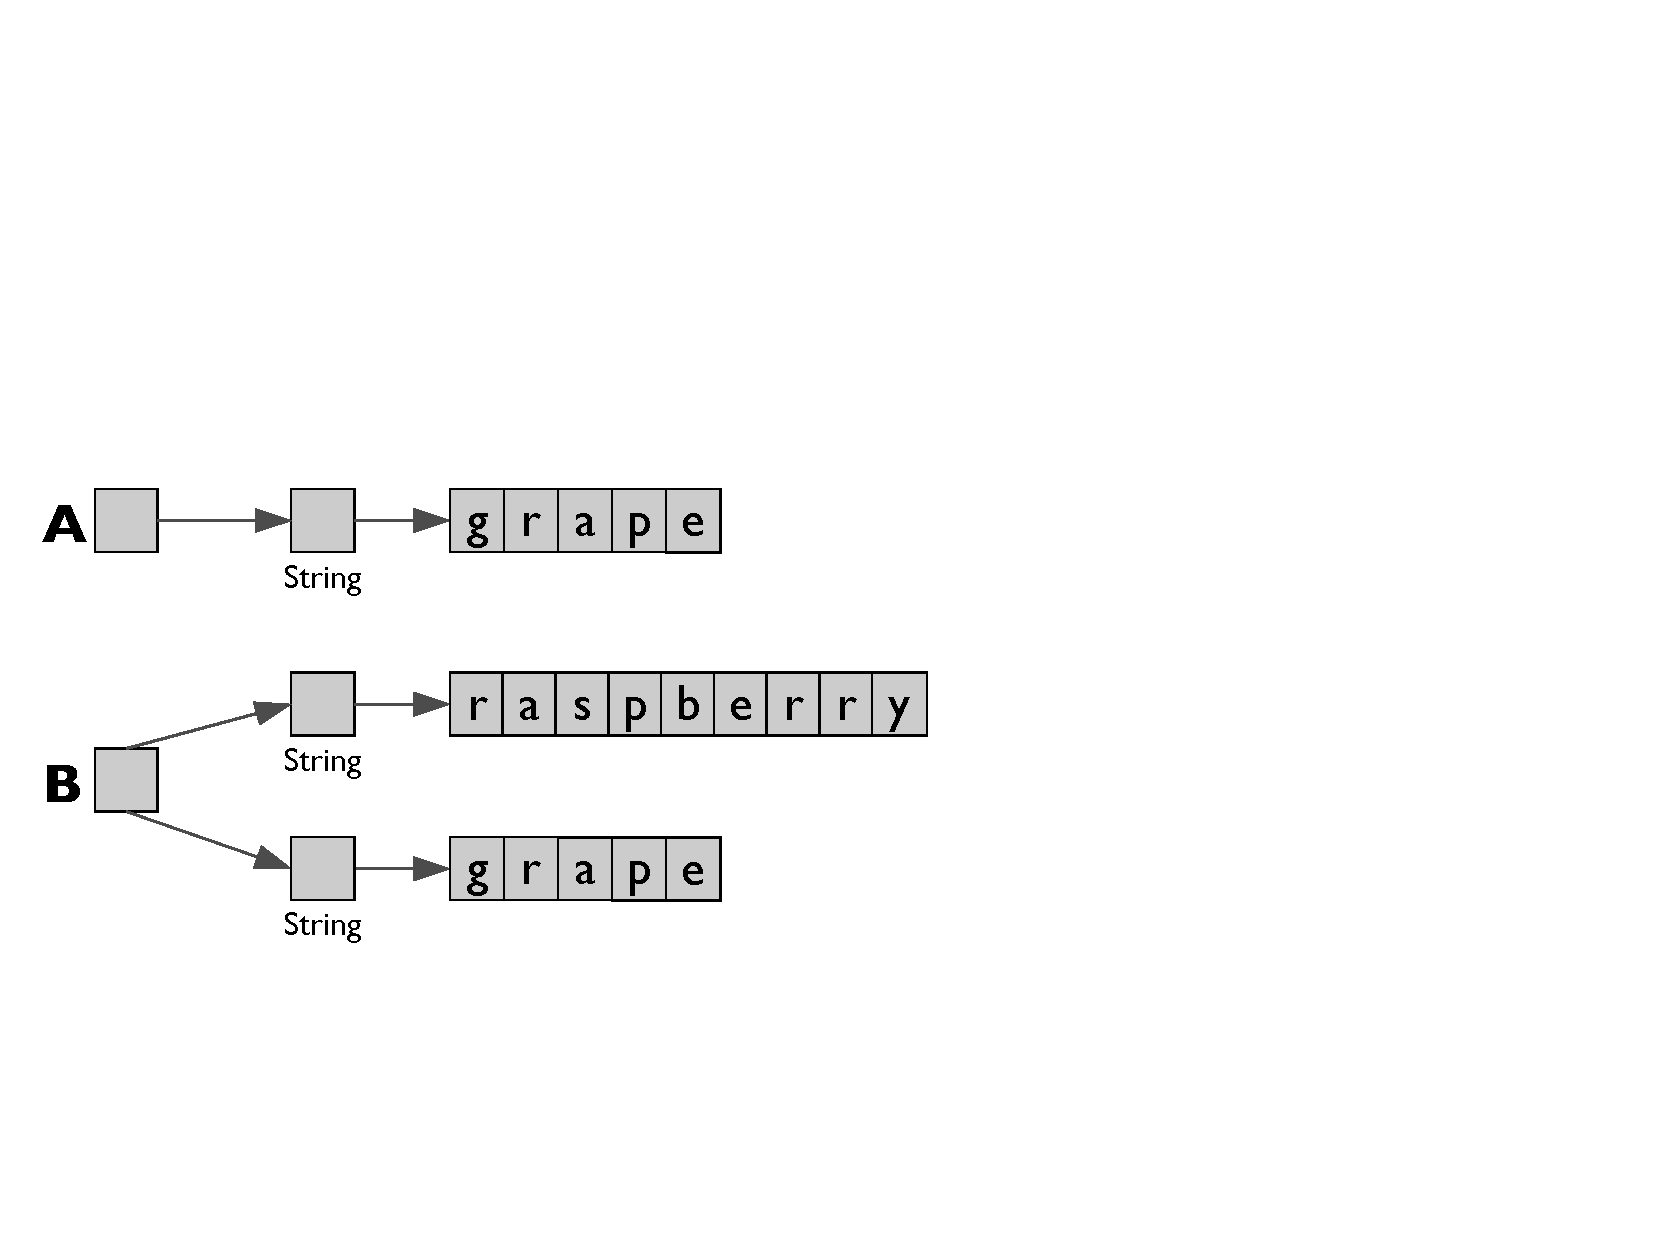
\includegraphics[width=0.425\textwidth]{part3/Figures/extreme/bulksharingpool1}}
	\qquad
	\subfigure[Interning.]{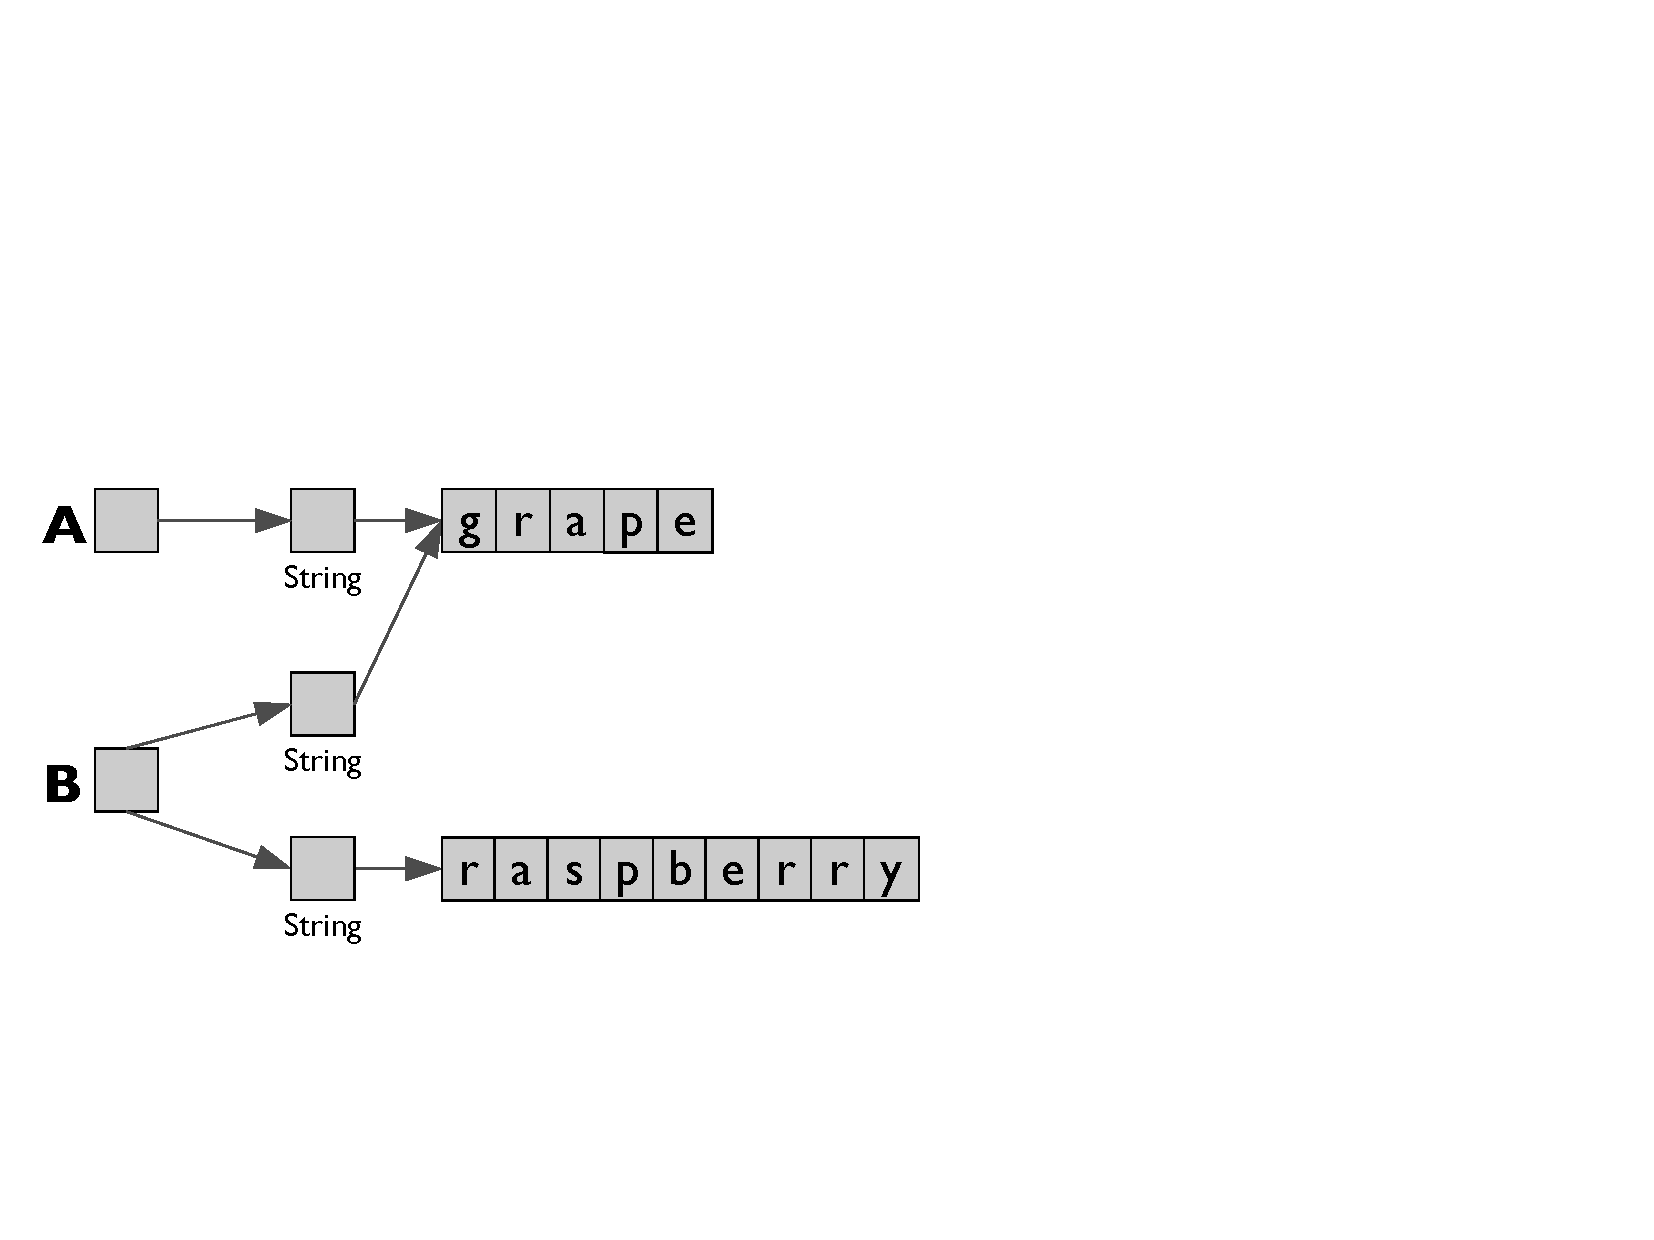
\includegraphics[width=0.425\textwidth]{part3/Figures/extreme/bulksharingpool2}}
	\qquad
	\subfigure[Bulk	sharing	pool.]{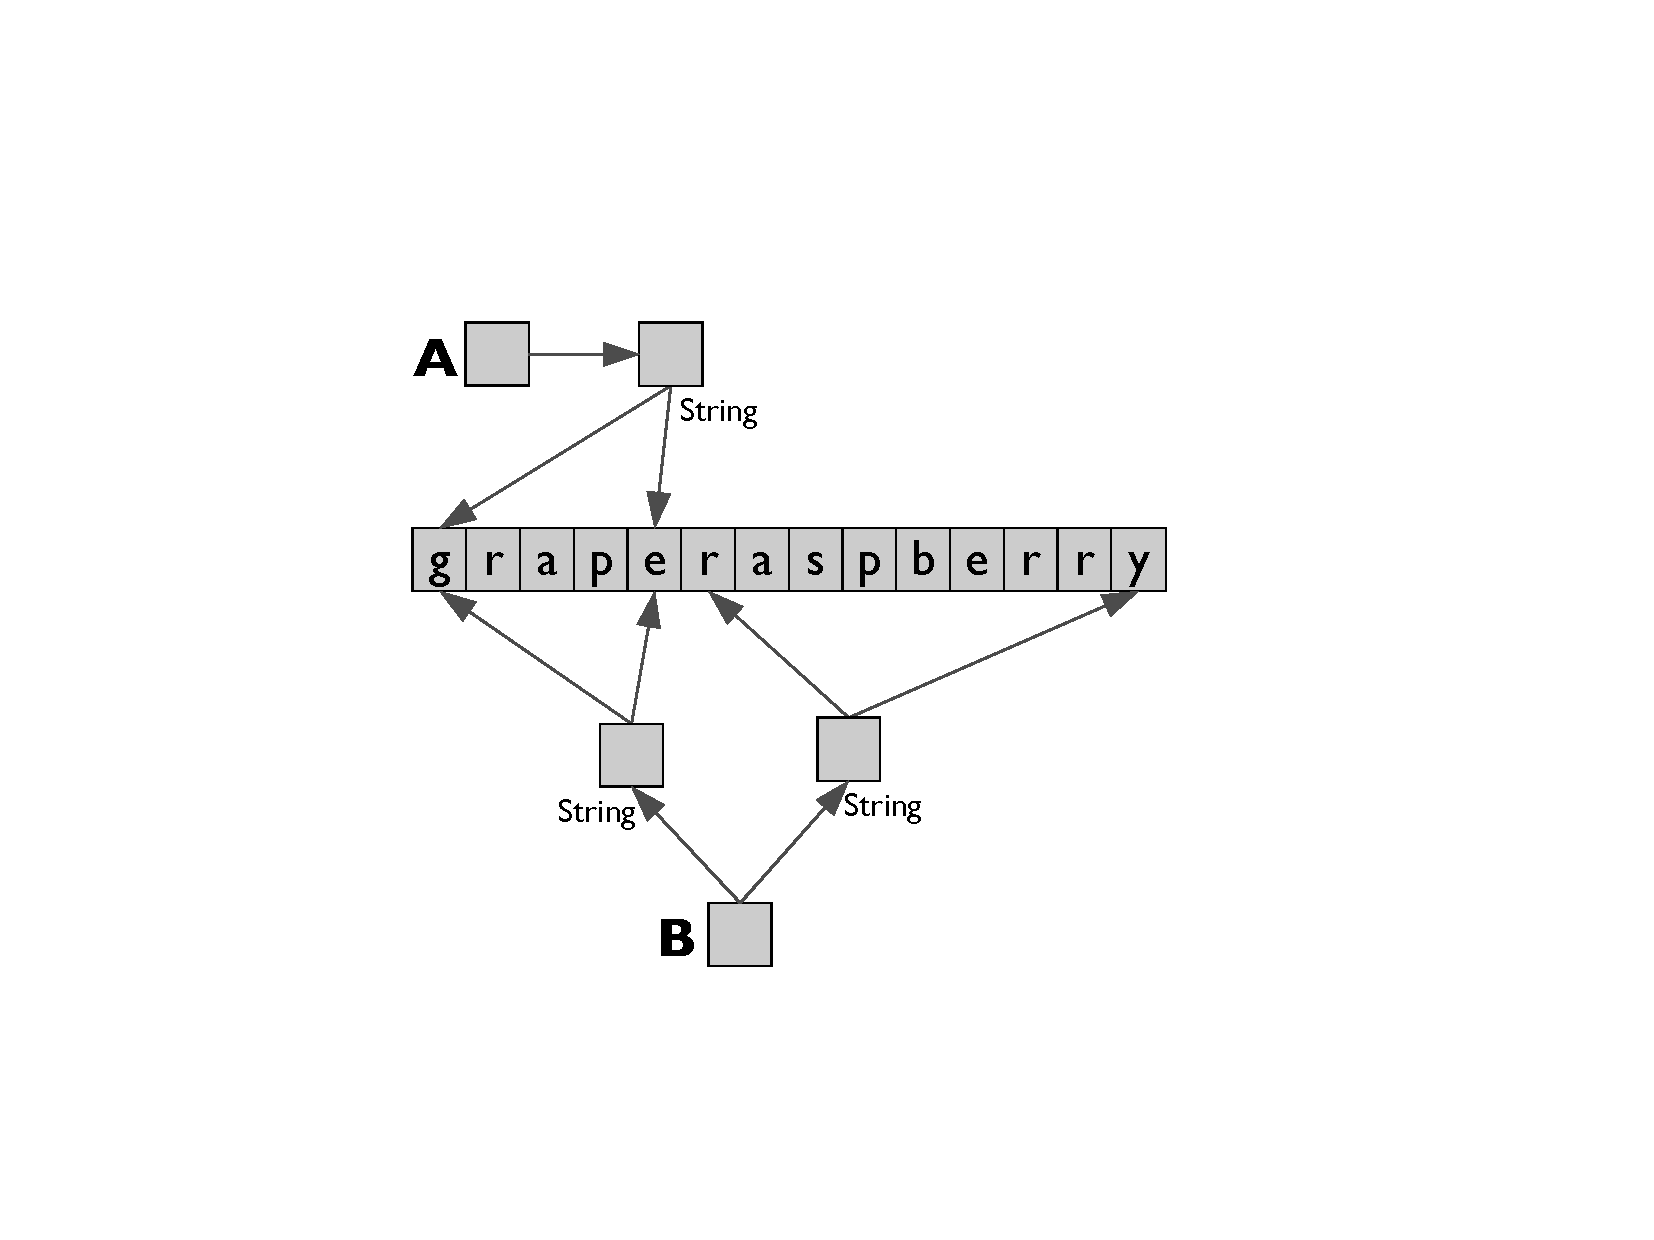
\includegraphics[width=0.36\textwidth]{part3/Figures/extreme/bulksharingpool3}}
	\qquad
	\subfigure[Bulk	sharing	pool, no wrappers.]{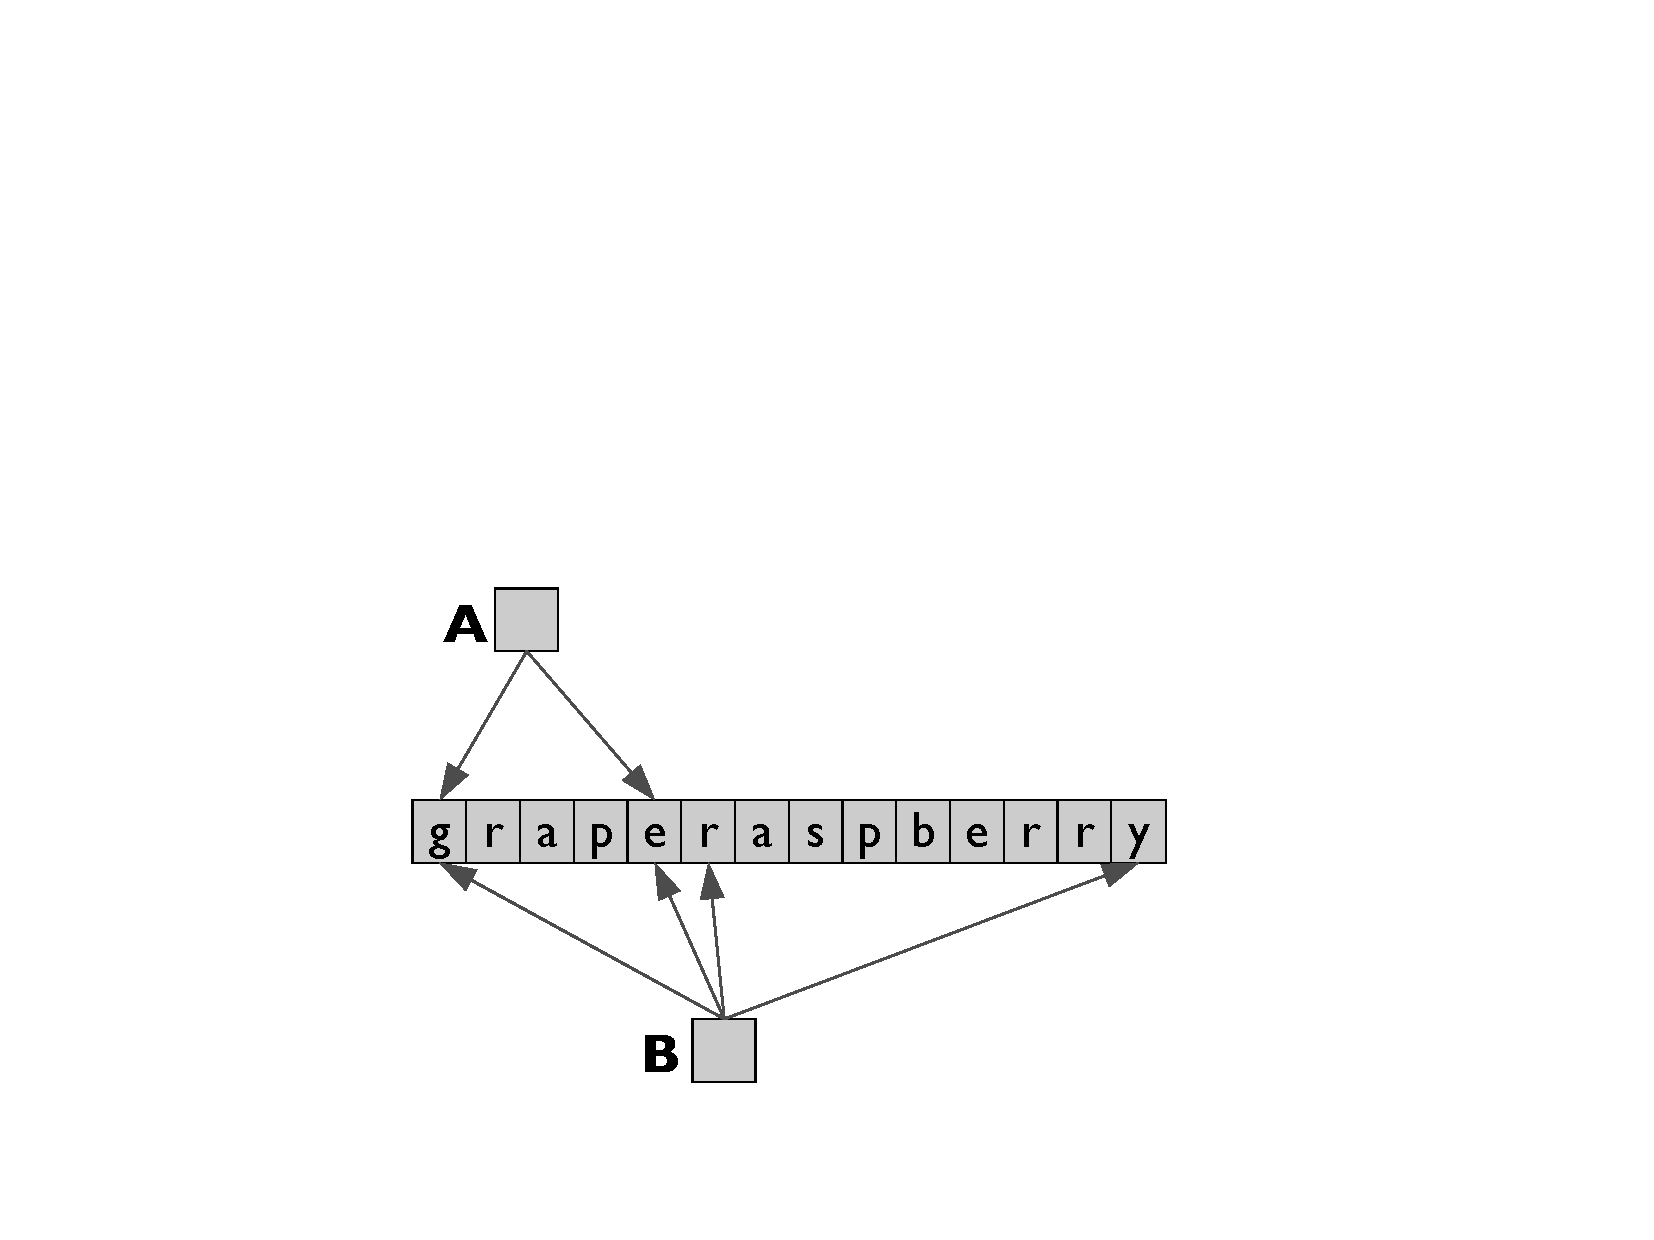
\includegraphics[width=0.36\textwidth]{part3/Figures/extreme/bulksharingpool4}}
	\subfigure[The memory consumed by one million strings, each of length 10
	bytes, for varying degrees of distinctness; e.g. 10\% means that
	there are only 100,000 distinct strings.]{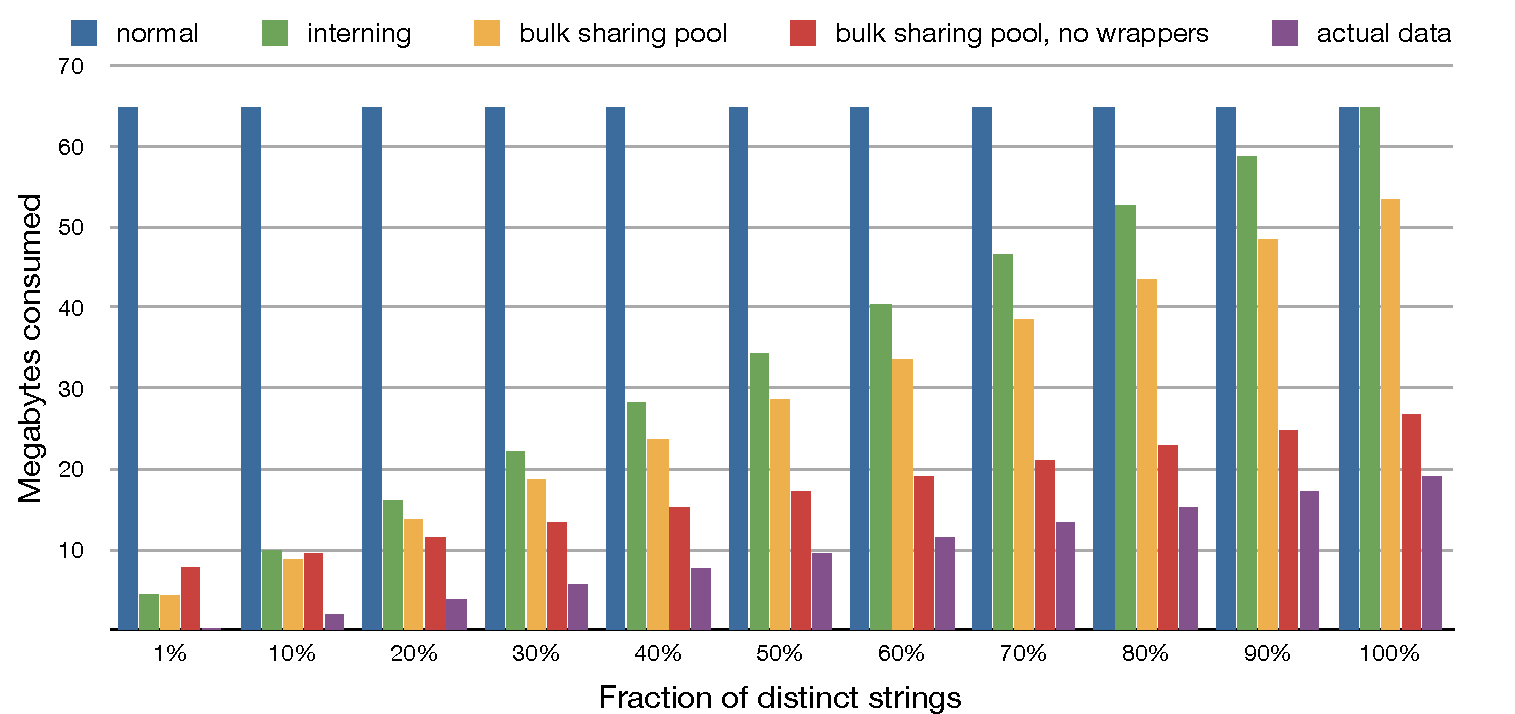
\includegraphics[width=\textwidth]{part3/Figures/extreme/bulksharingpool_consumptionchart.pdf}}
	\caption{If your application has many long-lived, but small, arrays of
	primitive data, it could suffer from high overhead. Interning avoids
	duplication. On top of interning, a Bulk Sharing Pool offers the additional
	potential for you to eliminate the primitive array wrappers, and so can be
	beneficial if there are still a large number of unique sequences.}
	\label{fig:bulk-sharing-pool}
\end{figure}


\begin{comment}
By eliminating many duplicates via interning, you stand to save a large amount of
memory, but your memory bloat factor will still be quite high. Instead of a bloat
factor of 83\%, with interning your heap will have a bloat factor of at least
88\%.
% 3*(16+32)/(10*2+3*(16+32))
This value is a lower bound, because there is another curious problem that arises
when handling duplicate data. If there is a bounded number of distinct sequences,
but an increasingly large number of total sequences, your memory bloat factor can
approach 100\%. In this case, the per-sequence memory overhead grows with the
number of sequences, but the amount of actual data is bounded by the number of
distinct sequences.
\end{comment}

\paragraph{Bulk Sharing Pools}

If you will never synchronize or reflect on sequences, as objects, then the
primitive array header and string wrapper are a needless expense. Another
possibility is to concatenate your many small arrays into fewer, longer, arrays.
\autoref{fig:bulk-sharing-pool}(c) illustrates this bulk storage of the
sequences in a single large array. You pay the primitive array overhead just
once, across all pooled sequences, rather than for every sequence.
% In this case, your heap will have a memory bloat factor of
% 3*(16+32)/(10*2+3*(16+32))

To achieve the ultimate in memory efficiency, you must also eliminate the
\class{String} wrapper objects, as shown in \autoref{fig:bulk-sharing-pool}(d).
This last step requires the most work on your part. If you have the luxury of
modifying the class definitions for the objects that contain the string
wrappers, then you can replace every pointer to a string with two numbers. These
numbers store indices into the single large array of bulk data, and demark the
sequence that the string wrapper would have contained. You are essentially
inlining the offset and length fields that every Java \class{String} object has,
and doing away with the hashcode field and the extra header and pointers. This
eliminates almost all sources of overhead.

This last, most extreme, optimization can reap large benefits in scalability,
but not always! You are paying an offset and length field in every object, even
when the strings are the same. For example, in
\autoref{fig:bulk-sharing-pool}(d), the offset and length fields for the two
uses of ``grape'' contain the same data. In the previous two optimizations,
these two fields are factored out into a separate \class{String} object, and so
only stored once. If the fraction of distinct strings
is small, then the cost of these duplicated fields outweighs the benefit of
removing the wrappers; it even outweighs the cost of removing the character
array headers. Where is the cross-over point?

\autoref{fig:bulk-sharing-pool}(e) shows the memory consumption of the four
implementations: using normal Java \class{Strings} without any attempt to remove
duplicates; using Java's built-in string interning mechiansm; using a bulk
sharing pool; and using a bulk sharing pool without any \class{String} wrappers.
The chart also includes a series comparison with the amount of memory consumed by
actual data.  The chart shows memory consumption of each implementation for
varying degrees of distinctness of the strings, for an case with one million
strings of length 10 characters each.
For example, if 500 thousand of the million strings are distinct (which
corresponds to the 50\% point in the chart), the normal implementation consumes
65 megabytes, the interning implementation consumes 34 megabytes, the bulk
sharing pool implementation consumes 27 megabytes, and the bulk implementation
without string wrappers consumes 17 megabytes. There are 500 thousand
distinct characters, so the actual data consumes about 10 megabytes. You can see
that the cross-over point, where the most extreme optimization begins to pay
off, occurs when about 10\% of the strings are distinct.

The chart shows just how much a few headers and pointers can affect the
scalability of your application. With only a bit of work, you can have an
implementation that scales very well, with only minimal overhead on top of the
actual data.





\section{When to Consider Using Bulk Storage}
\label{sec:when-bulk-storage-is-applicable}


The choice between bulk storage and using normal objects is analogous to the
choice between using an \class{ArrayList} versus a \class{LinkedList} to store a
list. An array-based list makes more efficient use of memory than its linked
counterpart, but does not support efficient insertion and deletion of random
list elements. Analogously, bulk storage removes all of the delegation links,
and stores data and relations in arrays. Removing an entity therefore entails
removing an entry from the arrays that stores the attributes of that type of
entity.

There are two main problems you will run into, with a column-oriented approach.
The first has been touched on briefly: the lack of strong typing for nodes and
edges. If everything is just an integer, your code will be buggy and hard to
maintain. Java does not have a facility for naming types, such as \code{typedef}
in the C language. The Java \code{enum} construct seems like it could help, but
this use case would require a permanent object for every node, and, besides,
this construct is limited to around 65,000 entries per enumeration. You can use transient
nodes, with some cost to performance, but your code must still obey an implicit
contract, one not enforced by the \code{javac} compiler, that reference equality
is never used on these transient facades.

The second problem centers around modifications to the node or edge model. This
style of storage works fantasically well, much better than normal Java objects,
for certain kinds of modifications. Adding attributes to models is easy.
Adding nodes is straigtforward. However, deleting nodes, and adding or
removing edges from existing nodes can only be done with some extra work. For
deletions, you would have to implement a form of garbage collection yourself.
Nodes and edges can be marked as deleted; deleted elements would be ignored by
normal access mechanisms. Adding edges to existing nodes is even more difficult.
For these reasons, it is highly recommended that you only employ column-oriented
storage for data structures that do not change in these ways.


 
\begin{comment}
also, the data doesn't need to be long-lived, that's an (also imprecise)
description of the preconditions under which the technique (bulk storage)
applies. it's also not read-mostly, because, with bulk storage, it's ok if the
attribute values change rapidly (in fact, things will probably be faster here,
due to cache locality), and it's also ok if the set of attributes changes (here
again bulk storage does a better job, much better in this case, than java). the
only thing that can't happen too much is deletion of entities.

3(you wrote, in your notes, "Is the data immutable", and "is it stable after a
point in time", neither of which is i think an absolute precondition of bulk
storage, or at least not that broadly; immutability only matters for the domain
of entities, but, even then, additions are OK, and even infrequent removals are
OK; or is this what you meant by "stability"?)
\end{comment}


\section{Summary}

\begin{itemize}
  \item Bulk storage is a technique for storing large volumes of data. It
  eliminates many of the usual overheads of storing objects, such as headers and
  delegation. Column-oriented storage is one way to store data in bulk form,
  and is well suited for use in Java applications. With this storage
  strategy, you can still program in Java and enjoy many of the benefits of the
  language, while simultaneusly enjoying large improvements in scalability.
  \item There are restrictions that will limit performance of column-oriented
  storage under certain circumstances. If the set of entities is in constant
  flux, then this strategy may not pay off.
  \item Your code quality will suffer somewhat. Entities are passed around as
  numbers, reducing the benefits of static type checking.
\end{itemize}


% Shortly, we will discuss the
%complexities, but benefits, of the latter style of API.

